% v2-acmtog-sample.tex, dated March 7 2012
% This is a sample file for ACM Transactions on Graphics
%
% Compilation using 'acmtog.cls' - version 1.2 (March 2012), Aptara Inc.
% (c) 2010 Association for Computing Machinery (ACM)
%
% Questions/Suggestions/Feedback should be addressed to => "acmtexsupport@aptaracorp.com".
% Users can also go through the FAQs available on the journal's submission webpage.
%
% Steps to compile: latex, bibtex, latex latex
%
% For tracking purposes => this is v1.2 - March 2012
\documentclass{sig-alternate} % v 2.5

% --- Author Metadata here ---
\conferenceinfo{Sample Conference}{'15 Potsdam, Germany}
%\CopyrightYear{2007} % Allows default copyright year (20XX) to be over-ridden - IF NEED BE.
%\crdata{0-12345-67-8/90/01}  % Allows default copyright data (0-89791-88-6/97/05) to be over-ridden - IF NEED BE.
% --- End of Author Metadata ---

\begin{document}

\title{Project Light}

\numberofauthors{5}

\author{
\alignauthor
Cornelius Bock
%
\alignauthor
Daniel Werner
%
\alignauthor
Felix Wolff
%
\and
\texttt{\{cornelius.bock|daniel.werner|felix.wolff\}@student.hpi.de} \\ \\
\and
\alignauthor
Christoph Meinel\\
    \affaddr{\textit{Supervisior}}
%
\alignauthor
Konrad-Felix Krentz\\
    \affaddr{\textit{Supervisior}}
}

\maketitle

\begin{abstract}
Lorem ipsum dolor sit amet, consectetur adipisicing elit, sed do eiusmod
tempor incididunt ut labore et dolore magna aliqua. Ut enim ad minim veniam,
quis nostrud exercitation ullamco laboris nisi ut aliquip ex ea commodo
consequat. Duis aute irure dolor in reprehenderit in voluptate velit esse
cillum dolore eu fugiat nulla pariatur. Excepteur sint occaecat cupidatat non
proident, sunt in culpa qui officia deserunt mollit anim id est laborum.
\end{abstract}

\category{K.6.5}{Management Of Computing And Information Systems}{Security}

\terms{Internet of Things, Security}

\keywords{awesome, keywords, go, here}

\section{Introduction}
\label{sec:introduction}

\begin{itemize}
	\item short introduction internet of things
	\item some words about contiki
	\item current security and key distribution situation (akes)
	\item idea of transmitting keying material using light and phone app, why light, alternative solutions
	\item setup (android device/app, mote with light sensor)
\end{itemize}


\section{Related Work}
\label{sec:related_work}

\begin{itemize}
	\item LiDSN: A Method to Deploy Wireless Sensor Networks Securely based on light communication
	\item ...
\end{itemize}


\section{Communication Protocol}
\label{sec:communication_protocol}

In the following section, we describe the phases of the protocol. 
Each phase contains the necessary steps for the Android device and the mote.
Insights into the concrete implementation will be given in the Section~\ref{sec:implementation}.

\subsection{Calibration}
\label{sub:calibration}

The goal of the calibration phase is to establish light values for \textit{bright} and \textit{dark} on the mote.
By doing this in the beginning of the protocol, we can adapt to different lighting situations in the room and different brightness levels of the phone.

The task of the phone in this protocol stage is simple. 
It periodically sends \textit{bright} and \textit{dark} values, each with a certain period length $T$.
Simply said, it is blinking.

The mote on the other side measures $n$ light values using its light sensor.
The time between two measurements will probably not be equal to $T$, because the period length is unknown to the mote at this point.
As long as \textit{bright} and \textit{dark} values are part of the $n$ measurements, the concrete time does not matter.
After reading $n$ values, the mote calculates reasonable numeric values for \textit{bright} and \textit{dark}.
For instance, this can be achieved by applying a \mbox{\textit{2-means}} algorithm, see Section~\ref{ssub:contiki_process}.
After that, the mote is able to classify new light values.
In other words, it can read bits.

\subsection{Synchronization}
\label{sub:synchronization}

During synchronization, the mote learns the period length $T$.
This is necessary to be able to read light values at the right time (see Figure~\ref{fig:read_a_bit}).

In this phase, the phone just keeps sending \textit{bright} and \textit{dark} values with the period length $T$.
This is the same as during calibration.

The mote on the other hand now measures light values as fast as it can and classifies them as \textit{0} and \textit{1}.
Once it notices that the bit flips, it records the time when the switch happened.
After recording $m$ bit flips, it can calculate the average period length.

With completion of the first two phases, the mote is now able to read data sent by the phone.
It learned a decision threshold for decoding the bits and the period length to read values at the right time.
Figure~\ref{fig:read_a_bit} shows how data can be read. 
However, the actual implementation slightly differs from that figure, see Section~\ref{sec:implementation}.

\begin{figure}
	\centering
	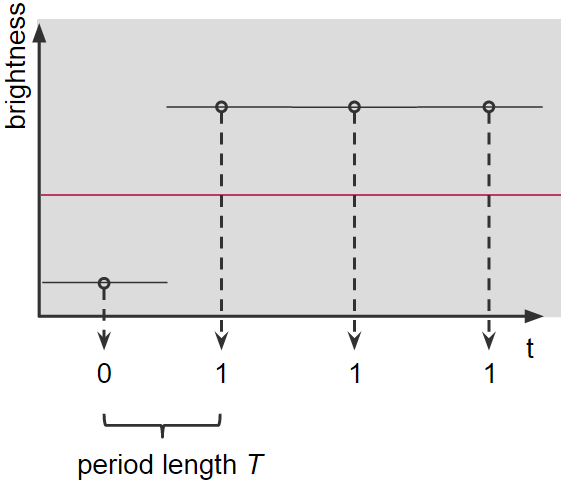
\includegraphics[scale=.5]{images/reading_data.png}
	\caption{Reading data: The black horizontal lines show the brightness emitted by the phone, the red line is the decision threshold for classifying \textit{0} and \textit{1}. Each arrow shows a point in time where the mote reads the value of the light sensor. The result here is the bit string 0111.}
	\label{fig:read_a_bit}
\end{figure}

\subsection{Initialization}
\label{sub:initialization}

\subsection{Data sending}
\label{sub:data_sending}

\subsection{Validation}
\label{sub:validation}



\section{Implementation}
\label{sec:implementation}

Project Light consists of an Android app that creates and sends the key material and a Contiki process that runs on the TelosB sky mote and receives and validates it.
Both follow the aforementioned communication protocol very closely, but increase reliability and fail-safeness through the following design decisions.

All data that is being sent is encoded using a Hamming(8,4)-code so that two-bit errors can be detected and one-bit errors can be corrected.

The CRC32 is chosen as the checksum algorithm for the validation phase to avoid saving erroneous key material.
This could be caused by 3-or-more-bit errors that the Hamming-code failed to detect.

As the android timer that triggers the bit "emission" cannot be too early but in fact tends to be a little late (cite android real time paper), the time at which the mote reads a bit is not in the middle of a period as suggested by Figure~\ref{fig:read_a_bit}.
It is at the very end of a period to maximize error avoidance due to "timer-lateness".

\subsection{Android app}
\label{sub:android_app}

functionality, flashlight, limitations

\subsection{Mote}
\label{sub:mote}

\subsubsection{Contiki process}
\label{ssub:contiki_process}

On the mote the communication protocol is implemented in a Contiki process.
The Contiki operating system offers a real-time timer called \textit{rtimer} which eliminates timer inaccuracies on the mote side.
The mote uses its light sensor to sense the current brightness.
Once the process is started an LED-countdown (red -> blue -> green) indicates the start of the key initialization procedure.
A \mbox{\textit{2-means}} algorithm is used to create two clusters of \textit{bright} and \textit{dark} values and to compute their mean values.
Subsequently a new value is classified as \textit{0} or \textit{1} depending on which mean value is closer to it.
After the successful synchronization and initialization a blue LED indicates that the mote is receiving data.
If an error is detected by the Hamming-code or if the computed checksum does not match the transmitted one, a red LED indidcates the failure and the process should be restarted.
A green LED shows that the key material has successfully been received and was saved to the permanent flash? memory of the mote.


\subsubsection{Contiki driver wrapper}
\label{ssub:contiki_driver_wrapper}

----- Maybe part about akes and how this fits together?! -----

For the mote to actually use the key material that was transmitted, the initialization of the link layer security needs to be delayed until that finished successfully.
To do so we created a link layer driver wrapper that accomplishes the following things:

\begin{itemize}
	\item "Delay"/Cancel all calls to the link layer driver.
	\item Check whether the key material was initialized before.
	\item If not, start the light process and wait for successful initialization.
	\item Forward all calls to the actual link layer driver.
\end{itemize}

As seen in (code example), calls to the driver that are being issued before the key material initialization are actually being canceled right now, but should eventually just be delayed and reissued once the initialization was finished.
Including the light app on a mote automatically redefines \textit{$NETSTACK\_CONF\_LLSEC$} to point to our link layer driver wrapper (and no further configuration needs to be done?).

\section{Results and Discussion}
\label{sec:results_and_discussion}

\begin{itemize}
	\item measure and evaluate maximum transmission speed, error rate
	\item is hamming code necessary (worth the doubled length) or CRC alone sufficient
	\item does the transmission rate have to be variable?
	\item "keep the phone busy" (wake up more often to prevent cpu from sleeping)
\end{itemize}



\section{Conclusion and Future Work}
\label{sec:future_work}

\begin{itemize}
	\item bidirectional communication using the LEDs of the mote (and maybe camera)
	\item 802.15.4 dongle to verify transmission (and do further initialization)
	\item initialize several mote together, separate synchronization and data sending
\end{itemize}

% Bibliography
\bibliographystyle{ACM-Reference-Format-Journals}
\bibliography{paper}

\end{document}
